The quality of the estimate produces by the estimation algorithm is limited by the quality of its input data, especially if the algorithm is not robust. In practice, sensor data can contain anomalous sensor samples, also called \textit{outliers}. While these samples might actually reflect reality, they usually stem from errors during measurement or transmission. In this section, the term \textit{outlier} will refer to bad samples that should be discarded, not surprising but correct samples which can occur in random processes. The challenge is to discern these two while minimizing the number of false positives (leads to discarding good measurements) and false negatives (degrades estimate quality). This improves estimation quality and can be crucial in safety-critical applications. This section presents common outlier types and methods to detect them.


\subsection{Outlier Types}\label{sec:outlier-types}
Outliers can be the result of a variety of issues. For example, heavy vibration and shocks might cause acceleration spikes and an optical cross-correlation sensor might see a featureless surface, so the recognized velocity drops to zero. In cabled transmission, a physical connection might be defect, while in radio transmission, the signal might drop out temporarily or there might be electromagnetic interference. Possible causes can vary a lot between environments, but a highly dynamic environment with many mechanical and electric parts such as an electric race car is likely to produce outliers at some point.

Outliers can be classified in four broad categories~\cites[p.~19]{Kabzan.2019}[p.~165~ff.]{Himmelblau.1994}, shown in figure~\ref{fig:outlier-types}:
\begin{itemize}
\item Spike/intermittent noise: a transient deviation from previous samples
\item Level shift: a transient deviation of the mean value
\item Drift/spurious trends: a slow variation of the mean value over time
\item Null/signal dropout: not receiving input or zero
\end{itemize}
Drift often occurs as the result of integrating a biased signal, e.g., caused by low frequency noise or temperature changes. The true mean does not change, but the accumulating error results in an observed trending mean. While there are other cases of poor data quality such as clipping and excessive noise, they rather stem from calibration problems and hardware errors, so they are not regarded further.

\begin{figure}[h]
	\begin{subfigure}[c]{0.5\textwidth}
		\centering
		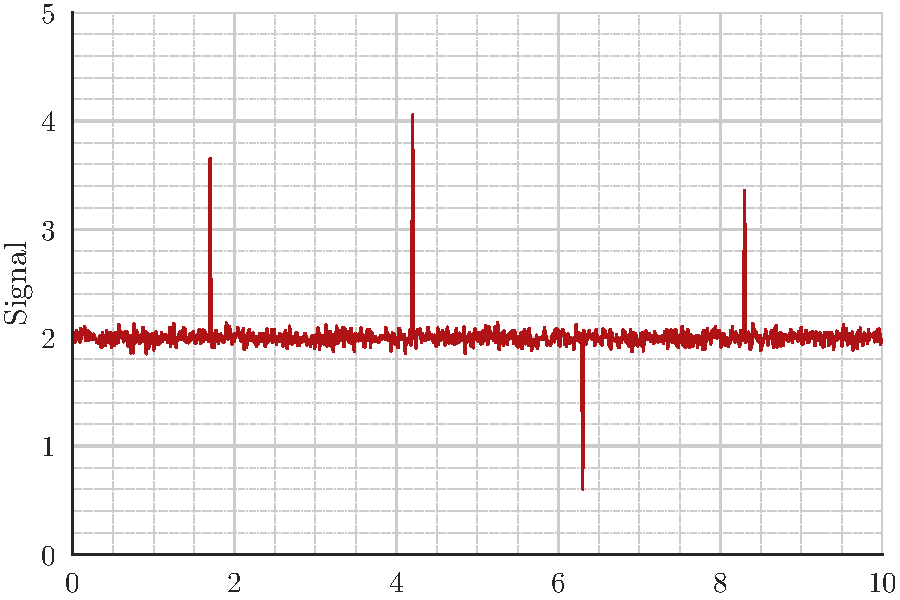
\includegraphics[width=0.95\textwidth]{plot_outlier_spike}%
		\subcaption{Spike}
		\label{fig:offcenter-spike}
	\end{subfigure}
	\begin{subfigure}[c]{0.5\textwidth}
		\centering
		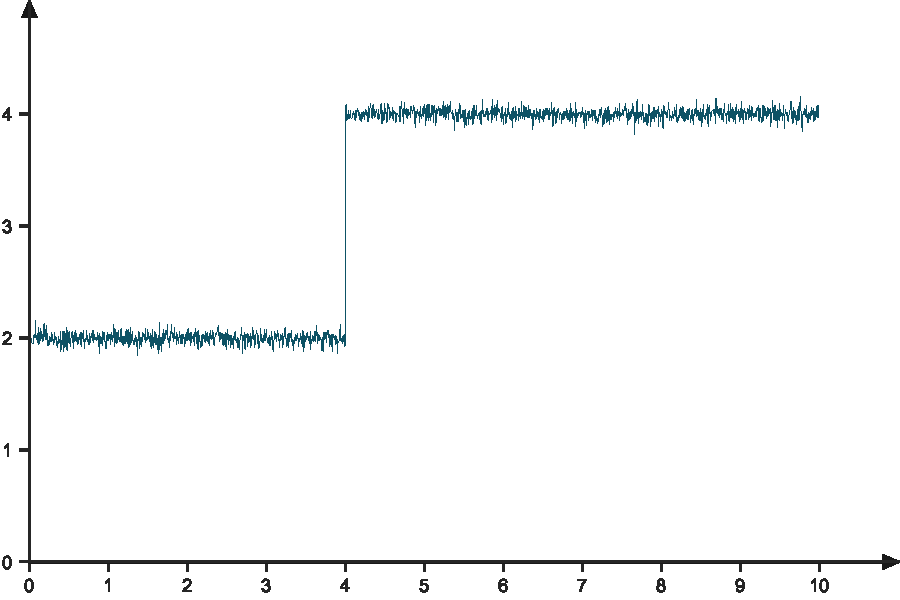
\includegraphics[width=0.95\textwidth]{plot_outlier_levelshift}%
		\subcaption{Level shift}
		\label{fig:outlier-type-levelshift}
	\end{subfigure}
	\begin{subfigure}[c]{0.5\textwidth}
		\centering
		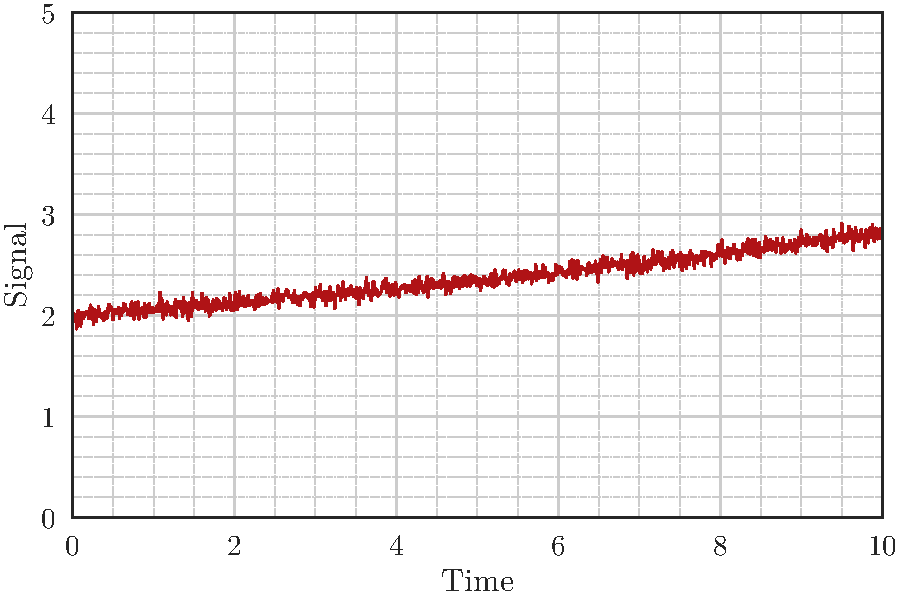
\includegraphics[width=0.95\textwidth]{plot_outlier_drift}%
		\subcaption{Drift}
		\label{fig:outlier-type-drift}
	\end{subfigure}
	\begin{subfigure}[c]{0.5\textwidth}
		\centering
		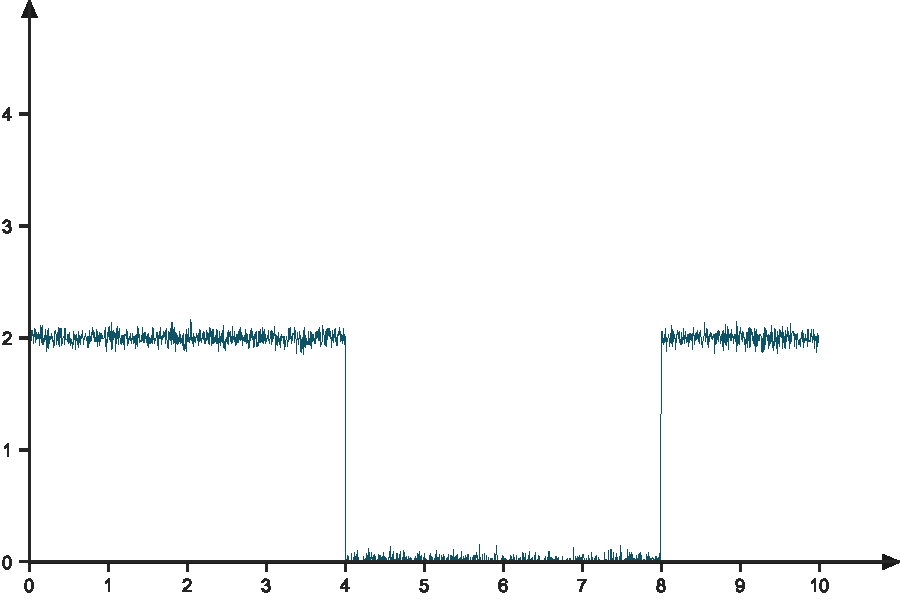
\includegraphics[width=0.95\textwidth]{plot_outlier_null}%
		\subcaption{Null}
		\label{fig:outlier-type-null}
	\end{subfigure}
	\caption{Outlier types}
	\label{fig:outlier-types}
\end{figure}

Outliers can be temporary or persistent. While spikes are inherently temporary, outliers of the other three categories might or might not return to normal. For example, a \gls{gps} signal can drop out because the sensor has no satellite connectivity for a couple of seconds but then recovers (as in figure \ref{fig:outlier-type-null}), while another sensor can be permanently damaged and will not recover (as in figure \ref{fig:outlier-type-levelshift}). Persistent but not transient outliers are hard to detect, and especially spurious trends cannot easily be distinguished from real trends by their nature. This motivates the need for two separate methods, an approach that is also employed by~\cite{Kabzan.2019}:
\begin{itemize}
\item A simple but strict method for transient outliers
\item A complex but lenient method for persistent outliers
\end{itemize}
With this dual approach, false negatives for easy-to-detect transient outliers can be minimized while false positives for hard-to-discern persistent outliers can be avoided. Note that the choice of detection thresholds influences the strictness and therefore sensitivity to a high degree.


\subsection{Rudimentary Methods}
Arguably the simplest method is the range check, shown in equation \ref{eq:outlier-range}. A plausible interval $[\tau_{min}, \tau_{max}]$ of values is defined in advance, and if the measurement $z$ is outside of that range, it is marked as outlier. For example, a speed of \SI{200}{\meter\per\second} is highly unlikely for a race car, and also high negative speeds are implausible.
\begin{equation}\label{eq:outlier-range}%
\tau_{min} < z < \tau_{max}%
\end{equation}

Another rudimentary method for detecting spikes is the difference of consecutive samples $z_t, z_{t-1}$, shown in equation \ref{eq:outlier-maxchangerate}. When the difference is higher than the maximum plausible change rate $\tau$, the current measurement is marked as outlier.
\begin{equation}\label{eq:outlier-maxchangerate}%
\abs{z_t - z_{t-1}} < \tau%
\end{equation}

Performing a sanity check is a good first approach to detect gross outliers. However, the thresholds should be set rather high to avoid false positives.


\subsection{Statistical Methods}\label{sec:outlier-statisticalmethods}
Methods based on the statistical properties of a signal can provide more granular checks than the previous rudimentary methods. One of the simplest robust statistics is the median, i.e. the center value when sorting a list of values, which is used in the method shown in equation \ref{eq:outlier-median}~\cite[p.~142]{Basu.2007}. An expected value $\tilde{z}_t$ is calculated using both the median of the last $k$ samples and the median of the differences of the last $k+1$ samples. If the difference between the expected and the actual value exceeds the threshold, the current sample is marked as outlier. The window size $k$ influences the robustness but also the detection delay, and should therefore be chosen carefully. Note that, once the outlier persists for more than $k$ samples, following measurements will be regarded as valid.
\begin{equation}\label{eq:outlier-median}%
\abs*{z_t - \underbrace{median(z_{t-k}, \ldots, z_{t-1}) + k \cdot median(z_{t-k} - z_{t-k-1}, \ldots, z_{t-1} - z_{t-2})}_\textrm{$\tilde{z}_t$}} < \tau%
\end{equation}

If an \gls{ekf} is used, a chi-squared test can be used to detect anomalies based on the residuals, as shown in equation \ref{eq:outlier-chisquared}~\cites[p.~4292]{Hausman.2016}[p.~2050~f.]{Valls.2018}. Since the residual $y$ is Gaussian distributed with the innovation covariance matrix $P_{yy}$ (for nomenclature, refer to section \ref{sec:background-ekf}), the normalized sum of squares of the residual values should be distributed according to a chi-squared distribution $\chi^2$ with as many degrees of freedom as there are measurements. An outlier is detected when the chi-squared test at a significance level of $\tau$ fails.
\begin{subequations}\label{eq:outlier-chisquared}
\begin{alignat}{2}%
y &= z - h(\hat{x}^-) \\%
P_{yy} &= H P^- H^T + R \\%
r^T P_{yy}^{-1} r &< \chi^2(\tau)%
\end{alignat}
\end{subequations}

Drift detection becomes easier when multiple sensors measure the same variable and can be compared. A simple variance-based approach based on this idea is shown in equation \ref{eq:outlier-variance}~\cite[p.~20]{Kabzan.2019}. For each time step, the summed variance of $n$ sensors is calculated, based on the mean $\mu_z$ of their measurements at that instant. Once the threshold $\tau \in (0, 1)$ is exceeded, the measurement with the highest contribution to the summed variance is marked as outlier.
\begin{equation}\label{eq:outlier-variance}%
\sum_{i=1}^n (z_i - \mu_z)^2 < \tau%
\end{equation}

The last approach we will regard in this chapter can be used for spike and drift detection, but requires $n>2$ sensors for a variable like the previous method. Multiple instances of the same \gls{ekf}, collectively called a bank of $n$ \gls{ekf}s, are executed in parallel. However, in the $i$-th filter, the measurement of the $i$-th sensor is disabled. In the event that an outlier in the $i$-th measurement occurs, all filters except the one that does not incorporate the faulty measurement will show a very high residual. \\ Equation \ref{eq:outlier-ekfbank}~\cite[p.~3]{Kobayashi.2003} shows how the sum of squared residuals\footnote{While the original paper talks about a \textit{weighted} sum of squared residuals, we omitted the weight coefficient in favor of an adjustable threshold.} $\textit{NSSR}^i$, normalized by the diagonal measurement covariance matrix $R^i$, is calculated from the residual $y_i$ of the $i$-th filter. The NSSR combines all elements of the residual vector into a single metric, enabling easy comparison with a threshold $\tau_i$. This threshold can be chosen empirically, or based on a desired statistical significance of the resulting $\chi^2$ distribution~\cite[p.~3]{Xue.2007}. Note that a more sophisticated approach to fault isolation, i.e. locating the sensor producing outliers, is required for the \gls{ekf} bank to work with multiple simultaneous outliers.
\begin{subequations}\label{eq:outlier-ekfbank}
\begin{alignat}{2}%
y^i &= z^i - h^i(\hat{x}^-) \\%
\underbrace{(y^i)^T (R^i)^{-1} y^i}_\textrm{$\textit{NSSR}^i$} &< \tau_i%
\end{alignat}
\end{subequations}
